%!Mode:: "TeX:UTF-8"

\section{代码:一些重要功能的C++实现}

\subsection{赋值函数}
\begin{lstlisting}[language=C++]
Widget& Widget::operator=(Widget& rhs)
{
	//not needed: if (*this == rhs) return *this;
	Widget temp(rhs);
	swap(temp);
	return *this;
}
\end{lstlisting}

\subsection{move函数}
\begin{lstlisting}[language=C++]
// move constructor  
    ArrayWrapper (ArrayWrapper&& other)  
        : _p_vals( other._p_vals  )  
        , _size( other._size )  
    {  
        other._p_vals = NULL;  
    }  
   
    // copy constructor  
    ArrayWrapper (const ArrayWrapper& other)  
        : _p_vals( new int[ other._size  ] )  
        , _size( other._size )  
    {  
        for ( int i = 0; i < _size; ++i )  
        {  
            _p_vals[ i ] = other._p_vals[ i ];  
        }  
    }  
\end{lstlisting}


\subsection{重载输入输出}


输入操作符的重载比和输出操作符复杂:输入操作符必须处理错误和文件结束的可能性。
\begin{lstlisting}[language=C++]

ostream& operator<<(ostream& out, const Sales_item& s)
{
	out << s.isbn << "\t" << s.units_sold << "\t"
		<< s.revenue << "\t" << s.avg_price();
	return out;
}

istream& operator>>(istream& in, Sales_item& s)
{
	double price;
	in >> s.isbn >> s.units_sold >> price;
	// check that the inputs succeeded
	if (in)
		s.revenue = s.units_sold * price;
	else
		s = Sales_item(); // input failed: reset object to default state
	return in;
}

\end{lstlisting}

\subsection{String类实现}
陈硕在酷壳发表了如下写法,适合面试。但是这段代码未实现追加操作。另外,strlen参数未判断是否为NULL,会导致未定义行为,
可改为\verb$str?strlen(str):0$。

\lstinputlisting{src/string-imp-chenhao.cpp}

实现2:
\lstinputlisting{src/string-imp-2.cpp}

实现3:
\lstinputlisting{src/string-imp-3.cpp}

\subsection{智能指针}

C++98 \verb$auto_ptr$的缺陷:功能缺失(构造函数的move语义,赋值操作符),导致不易理解,容易出错。
标准容器不能容纳\verb$auto_ptr$,因为它的转移语义。

\verb$shared_ptr$的循环引用会导致内存泄露。改用弱引用可打破这个循环。
\verb$weak_ptr$为弱引用,而\verb$shared_ptr$为强引用。
\verb$weak_ptr$除了对所管理对象的基本访问功能(通过get()函数)外,还有两个常用的功能函数:expired()用于检测所管理的对象是否已经释放;lock()用于获取所管理的对象的强引用指针。
当expired()为true的时候,lock()函数将返回一个存储空指针的\verb$shared_ptr$。

\verb$auto_ptr$代码示例如下:
\lstinputlisting{src/autoptr.cpp}

\subsection{引用计数}

计数方法的实现有2种,内置和外置。
内置指的是对象本身就有计数功能,也就是计数的值变量是对象的成员;
外置则是指对象本身不需要支持计数功能,我们是在外部给它加上这个计数能力的。

\begin{figure}[ht]
	\begin{center}
		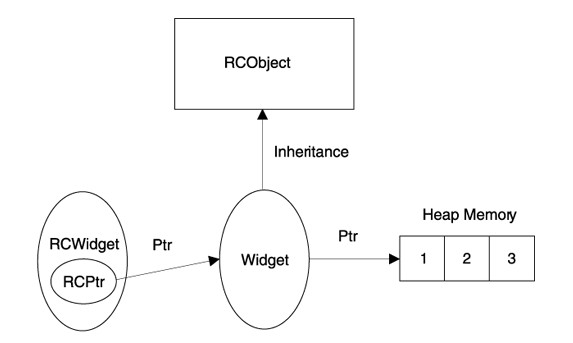
\includegraphics[keepaspectratio,width=0.4\paperwidth]{Pictures/RCObject.jpg}
	\caption{内置引用计数}
	\label{fig:RCObject}
	\end{center}
\end{figure}

\begin{figure}[ht]
	\begin{center}
		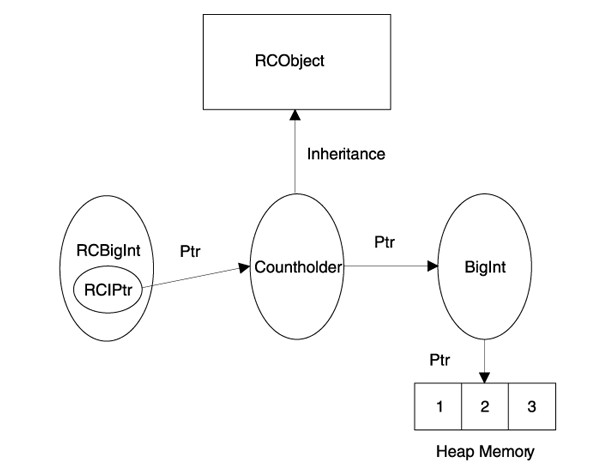
\includegraphics[keepaspectratio,width=0.4\paperwidth]{Pictures/RCObject-out.jpg}
	\caption{外置引用计数}
	\label{fig:RCObject}
	\end{center}
\end{figure}

内置引用计数示例代码:
\lstinputlisting{src/refcount.cpp}



\clearpage















